\documentclass[11pt,letterpaper]{article}
\usepackage[T1]{fontenc}
\usepackage[scaled]{helvet}
\renewcommand{\familydefault}{\sfdefault}
\usepackage{amsmath,amssymb}
\usepackage[margin=0.8in,bottom=0.9in]{geometry}
\usepackage[most]{tcolorbox}
\usepackage{tikz}
\usetikzlibrary{calc}
\usepackage{enumitem}
\usepackage{array}
\usepackage{needspace}
\usepackage{fancyhdr}
\usepackage{pifont}

% ---- Palette "F. Bright & Playful" ----
\definecolor{fmtitle}{HTML}{3D2C8D}
\definecolor{fmkey}{HTML}{0096C7}
\definecolor{fmwatch}{HTML}{2BB673}
\definecolor{fmturn}{HTML}{F4A100}
\definecolor{fmmistake}{HTML}{EF476F}
\definecolor{fmnotice}{HTML}{9B5DE5}
\definecolor{fmgray}{HTML}{6B6B6B}

\pagestyle{fancy}
\fancyhf{}
\renewcommand{\headrulewidth}{0pt}
\fancyfoot[C]{\footnotesize\color{fmgray}\textcopyright\ 2026 FangMath. All rights reserved.}
\fancyfoot[R]{\footnotesize\color{fmgray}\thepage}
\setlength{\parindent}{0pt}
\setlength{\parskip}{3pt}

\newcommand{\badge}[1]{\colorbox{fmtitle}{\color{white}\bfseries\small\ #1\ }}
\newcommand{\leveltag}[2]{\colorbox{#1}{\color{white}\bfseries\scriptsize\ #2\ }}
\newcommand{\LE}{\leveltag{fmwatch}{EASY}}
\newcommand{\LM}{\leveltag{fmturn}{MEDIUM}}
\newcommand{\LH}{\leveltag{fmmistake}{HARD}}

\newcommand{\sectionbar}[2]{\needspace{6cm}\par\vspace{4mm}
  \begin{tcolorbox}[enhanced,colback=fmtitle,colframe=fmtitle,arc=2mm,
    left=4mm,top=1.5mm,bottom=1.5mm]
  \color{white}\bfseries\large #1\hfill{\normalsize\mdseries #2}
  \end{tcolorbox}}

\newtcolorbox{keyidea}{enhanced,breakable,colback=white,colframe=fmkey,boxrule=1pt,arc=2mm,
  title={Key Idea},coltitle=fmkey,fonttitle=\bfseries,
  attach boxed title to top left={xshift=4mm,yshift=-2mm},
  boxed title style={colback=white,colframe=fmkey,boxrule=0.9pt}}
\newtcolorbox{watchme}{enhanced,colback=white,colframe=fmwatch,boxrule=1pt,arc=2mm,
  title={Watch Me --- Worked Example},coltitle=fmwatch,fonttitle=\bfseries,
  attach boxed title to top left={xshift=4mm,yshift=-2mm},
  boxed title style={colback=white,colframe=fmwatch,boxrule=0.9pt}}
\newtcolorbox{mistakebox}{enhanced,breakable,colback=white,colframe=fmmistake,boxrule=1pt,arc=2mm,
  title={Common Mistake},coltitle=fmmistake,fonttitle=\bfseries,
  attach boxed title to top left={xshift=4mm,yshift=-2mm},
  boxed title style={colback=white,colframe=fmmistake,boxrule=0.9pt}}
\newtcolorbox{yourturn}{enhanced,breakable,colback=white,colframe=fmturn,boxrule=1pt,arc=2mm,
  title={Your Turn},coltitle=fmturn,fonttitle=\bfseries,
  attach boxed title to top left={xshift=4mm,yshift=-2mm},
  boxed title style={colback=white,colframe=fmturn,boxrule=0.9pt}}
\newtcolorbox{answerbox}[1]{enhanced,breakable,colback=white,colframe=fmwatch,boxrule=1pt,arc=2mm,
  title={#1},coltitle=fmwatch,fonttitle=\bfseries,
  attach boxed title to top left={xshift=4mm,yshift=-2mm},
  boxed title style={colback=white,colframe=fmwatch,boxrule=0.9pt}}

\newcommand{\work}[1]{\par\vspace{#1}}
\setlist[enumerate]{itemsep=2pt,topsep=3pt}

% ---------------- extra boxes ----------------
\newtcolorbox{notebox}{enhanced,breakable,colback=white,colframe=fmnotice,boxrule=1pt,arc=2mm,
  title={Notice},coltitle=fmnotice,fonttitle=\bfseries,
  attach boxed title to top left={xshift=4mm,yshift=-2mm},
  boxed title style={colback=white,colframe=fmnotice,boxrule=0.9pt}}
\newtcolorbox{exbox}{enhanced,colback=white,colframe=fmwatch,boxrule=0.8pt,arc=2mm,
  title={Example},coltitle=fmwatch,fonttitle=\bfseries\small,
  attach boxed title to top left={xshift=4mm,yshift=-2mm},
  boxed title style={colback=white,colframe=fmwatch,boxrule=0.8pt},fontupper=\small}
\newcommand{\topicbar}[1]{\needspace{4.5cm}\par\vspace{5mm}
  \begin{tcolorbox}[enhanced,colback=fmtitle,colframe=fmtitle,arc=2mm,left=4mm,top=1.5mm,bottom=1.5mm]
  \color{white}\bfseries\large #1
  \end{tcolorbox}}
\usepackage{multicol}

% ---------------- practice layout ----------------
\newcommand{\workline}{\par\vspace{7mm}{\color{gray!55}\rule{\linewidth}{0.4pt}}}
\newcommand{\worklines}[1]{\foreach \i in {1,...,#1}{\workline}}
\newcommand{\prob}[3]{\needspace{#3}\par\vspace{3mm}{\color{fmturn}\bfseries #1.}\ #2\par}
\newcommand{\ansline}{\par\vspace{4mm}\hfill\textbf{Answer:}\ \rule{5cm}{0.4pt}\par}
\newcommand{\keyitem}[3]{\needspace{3.2cm}\par\vspace{2mm}
  \begin{tcolorbox}[enhanced,colback=white,colframe=fmwatch!60,boxrule=0.6pt,arc=1.5mm,left=3mm,top=1.5mm,bottom=1.5mm]
  {\color{fmwatch}\bfseries #1.}\quad\small #2\par\vspace{1mm}
  \normalsize\textbf{Answer: #3}
  \end{tcolorbox}}



\newcommand{\grid}[1][0.32]{\begin{tikzpicture}[scale=#1]
 \draw[gray!30,thin] (-6,-6) grid (6,6);
 \draw[->,thick] (-6.4,0)--(6.5,0) node[right,font=\scriptsize]{$x$};
 \draw[->,thick] (0,-6.4)--(0,6.5) node[above,font=\scriptsize]{$y$};
 
\end{tikzpicture}}

\begin{document}
\badge{WORKSHEET}\hfill{\small\color{fmgray}Algebra 1 \textperiodcentered\ Linear Functions}\par\vspace{4mm}
{\color{fmtitle}\LARGE\bfseries Linear Functions \& Graphing}\par\vspace{1mm}
{\color{fmgray}30 problems \textperiodcentered\ A worked example comes before each type. Show every step.}\par\vspace{3mm}
Name: \rule{6cm}{0.4pt}\hspace{1cm}Date: \rule{3.5cm}{0.4pt}\par\vspace{1mm}

\begin{keyidea}A \textbf{linear function} makes a straight line. Two numbers tell you everything about it:
\begin{itemize}[itemsep=1pt,topsep=2pt]
\item the \textbf{slope} $m = \dfrac{\text{rise}}{\text{run}} = \dfrac{y_2 - y_1}{x_2 - x_1}$ \ --- how steep the line is, and which way it goes;
\item the \textbf{$y$-intercept} $b$ \ --- where the line crosses the $y$-axis, the point $(0, b)$.
\end{itemize}
Put together: \textbf{slope-intercept form} $y = mx + b$.\end{keyidea}
\begin{mistakebox}Keep the same order on top and bottom: $\dfrac{y_2 - y_1}{x_2 - x_1}$, \textbf{not} $\dfrac{y_2 - y_1}{x_1 - x_2}$.\par
In $y = mx + b$, $y$ must be alone first. In $2y = 4x + 6$ the slope is $2$, \textbf{not} $4$: divide everything by 2 to get $y = 2x + 3$.\end{mistakebox}
\needspace{9cm}\topicbar{Type 1 \quad Slope from Two Points}
\begin{watchme}\textbf{Find the slope of the line through $(1, 2)$ and $(4, 8)$.}\par\vspace{1mm}Rise over run: how much $y$ changes, divided by how much $x$ changes.\par\vspace{1mm}
\renewcommand{\arraystretch}{2.0}\begin{tabular}{@{}l l@{}}
\textbf{Step 1 \ Subtract the $y$'s} & $8 - 2 = 6$\\
\textbf{Step 2 \ Subtract the $x$'s (same order)} & $4 - 1 = 3$\\
\textbf{Answer} & $\boldsymbol{m = \dfrac{6}{3} = 2}$
\end{tabular}\end{watchme}
\needspace{3.1cm}\par\vspace{3mm}\noindent \begin{minipage}[t][2.6cm]{0.48\linewidth}\raggedright{\color{fmturn}\bfseries 1.}\ Find the slope through $(2, 3)$ and $(4, 7)$.\par\vfill\hfill $m =$\ \rule{3.2cm}{0.4pt}\end{minipage}\hfill \begin{minipage}[t][2.6cm]{0.48\linewidth}\raggedright{\color{fmturn}\bfseries 2.}\ Find the slope through $(1, 5)$ and $(3, 1)$.\par\vfill\hfill $m =$\ \rule{3.2cm}{0.4pt}\end{minipage}\par
\needspace{3.1cm}\par\vspace{3mm}\noindent \begin{minipage}[t][2.6cm]{0.48\linewidth}\raggedright{\color{fmturn}\bfseries 3.}\ Find the slope through $(-2, 4)$ and $(2, 6)$.\par\vfill\hfill $m =$\ \rule{3.2cm}{0.4pt}\end{minipage}\hfill \begin{minipage}[t][2.6cm]{0.48\linewidth}\raggedright{\color{fmturn}\bfseries 4.}\ Find the slope through $(0, -3)$ and $(5, -3)$.\par\vfill\hfill $m =$\ \rule{3.2cm}{0.4pt}\end{minipage}\par
\needspace{3.1cm}\par\vspace{3mm}\noindent \begin{minipage}[t][2.6cm]{0.48\linewidth}\raggedright{\color{fmturn}\bfseries 5.}\ Find the slope through $(-4, -1)$ and $(2, 8)$.\par\vfill\hfill $m =$\ \rule{3.2cm}{0.4pt}\end{minipage}\hfill \begin{minipage}[t][2.6cm]{0.48\linewidth}\raggedright{\color{fmturn}\bfseries 6.}\ Find the slope through $(3, 2)$ and $(3, 7)$.\par\vfill\hfill $m =$\ \rule{3.2cm}{0.4pt}\end{minipage}\par
\needspace{9cm}\topicbar{Type 2 \quad Slope from a Graph}
\begin{watchme}\textbf{Find the slope of the line in the graph.}\par\vspace{1mm}\begin{minipage}[c]{0.55\linewidth}Pick two points where the line crosses grid corners: $(0, -1)$ and $(2, 3)$. Count from the left point to the right point.\par\vspace{1mm}Up $4$ (rise), right $2$ (run).\par\vspace{1mm}\textbf{Answer} \ $\boldsymbol{m = \dfrac{4}{2} = 2}$. \ Going up to the right means a \textbf{positive} slope.\end{minipage}\hfill\begin{minipage}[c]{0.4\linewidth}\centering 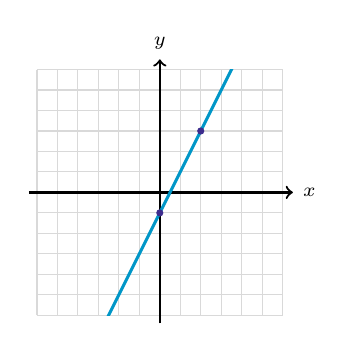
\begin{tikzpicture}[scale=0.26]
\draw[gray!30,thin] (-6,-6) grid (6,6);
\draw[->,thick] (-6.4,0)--(6.5,0) node[right,font=\scriptsize]{$x$};
\draw[->,thick] (0,-6.4)--(0,6.5) node[above,font=\scriptsize]{$y$};
\begin{scope}\clip (-6,-6) rectangle (6,6);
\draw[fmkey,line width=1.1pt] (-7,-15.000)--(7,13.000);
\end{scope}
\fill[fmtitle] (0.0,-1.0) circle (5pt);
\fill[fmtitle] (2.0,3.0) circle (5pt);
\end{tikzpicture}\end{minipage}\end{watchme}
\needspace{6.6cm}\par\vspace{3mm}\noindent \begin{minipage}[t]{0.48\linewidth}\raggedright{\color{fmturn}\bfseries 7.}\ Find the slope of the line.\par\vspace{1mm}\centering 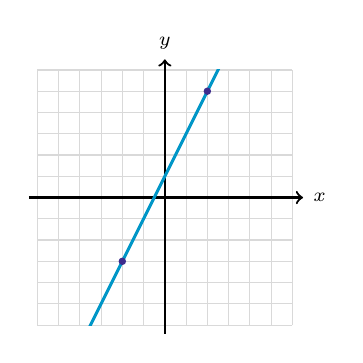
\begin{tikzpicture}[scale=0.27]
\draw[gray!30,thin] (-6,-6) grid (6,6);
\draw[->,thick] (-6.4,0)--(6.5,0) node[right,font=\scriptsize]{$x$};
\draw[->,thick] (0,-6.4)--(0,6.5) node[above,font=\scriptsize]{$y$};
\begin{scope}\clip (-6,-6) rectangle (6,6);
\draw[fmkey,line width=1.1pt] (-7,-13.000)--(7,15.000);
\end{scope}
\fill[fmtitle] (-2.0,-3.0) circle (5pt);
\fill[fmtitle] (2.0,5.0) circle (5pt);
\end{tikzpicture}\par\vspace{2mm}\raggedleft $m =$\ \rule{3.2cm}{0.4pt}\end{minipage}\hfill \begin{minipage}[t]{0.48\linewidth}\raggedright{\color{fmturn}\bfseries 8.}\ Find the slope of the line.\par\vspace{1mm}\centering 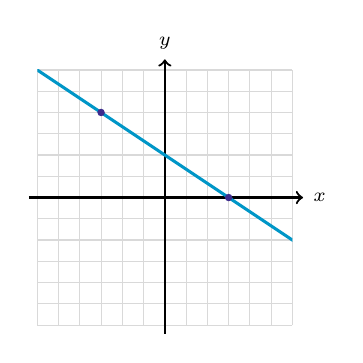
\begin{tikzpicture}[scale=0.27]
\draw[gray!30,thin] (-6,-6) grid (6,6);
\draw[->,thick] (-6.4,0)--(6.5,0) node[right,font=\scriptsize]{$x$};
\draw[->,thick] (0,-6.4)--(0,6.5) node[above,font=\scriptsize]{$y$};
\begin{scope}\clip (-6,-6) rectangle (6,6);
\draw[fmkey,line width=1.1pt] (-7,6.667)--(7,-2.667);
\end{scope}
\fill[fmtitle] (-3.0,4.0) circle (5pt);
\fill[fmtitle] (3.0,0.0) circle (5pt);
\end{tikzpicture}\par\vspace{2mm}\raggedleft $m =$\ \rule{3.2cm}{0.4pt}\end{minipage}\par
\needspace{6.6cm}\par\vspace{3mm}\noindent \begin{minipage}[t]{0.48\linewidth}\raggedright{\color{fmturn}\bfseries 9.}\ Find the slope of the line.\par\vspace{1mm}\centering 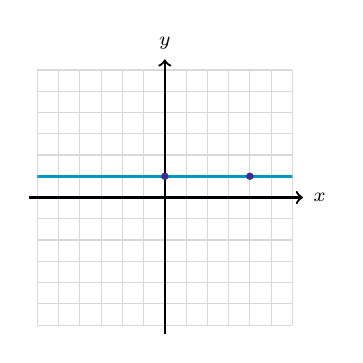
\begin{tikzpicture}[scale=0.27]
\draw[gray!30,thin] (-6,-6) grid (6,6);
\draw[->,thick] (-6.4,0)--(6.5,0) node[right,font=\scriptsize]{$x$};
\draw[->,thick] (0,-6.4)--(0,6.5) node[above,font=\scriptsize]{$y$};
\begin{scope}\clip (-6,-6) rectangle (6,6);
\draw[fmkey,line width=1.1pt] (-7,1.000)--(7,1.000);
\end{scope}
\fill[fmtitle] (0.0,1.0) circle (5pt);
\fill[fmtitle] (4.0,1.0) circle (5pt);
\end{tikzpicture}\par\vspace{2mm}\raggedleft $m =$\ \rule{3.2cm}{0.4pt}\end{minipage}\hfill \begin{minipage}[t]{0.48\linewidth}\raggedright{\color{fmturn}\bfseries 10.}\ Find the slope of the line.\par\vspace{1mm}\centering 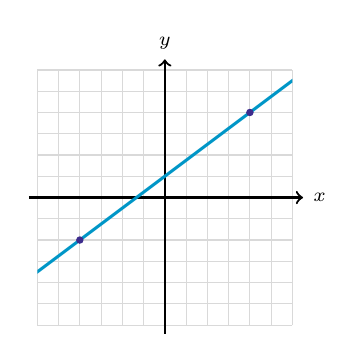
\begin{tikzpicture}[scale=0.27]
\draw[gray!30,thin] (-6,-6) grid (6,6);
\draw[->,thick] (-6.4,0)--(6.5,0) node[right,font=\scriptsize]{$x$};
\draw[->,thick] (0,-6.4)--(0,6.5) node[above,font=\scriptsize]{$y$};
\begin{scope}\clip (-6,-6) rectangle (6,6);
\draw[fmkey,line width=1.1pt] (-7,-4.250)--(7,6.250);
\end{scope}
\fill[fmtitle] (-4.0,-2.0) circle (5pt);
\fill[fmtitle] (4.0,4.0) circle (5pt);
\end{tikzpicture}\par\vspace{2mm}\raggedleft $m =$\ \rule{3.2cm}{0.4pt}\end{minipage}\par
\needspace{9cm}\topicbar{Type 3 \quad Intercepts}
\begin{watchme}\textbf{Find the $x$- and $y$-intercepts of $2x + 3y = 12$.}\par\vspace{1mm}On the $x$-axis, $y = 0$. On the $y$-axis, $x = 0$.\par\vspace{1mm}
\renewcommand{\arraystretch}{2.0}\begin{tabular}{@{}l l@{}}
\textbf{$x$-intercept \ Let $y = 0$} & $2x = 12$, \ $x = 6$ \ $\to (6, 0)$\\
\textbf{$y$-intercept \ Let $x = 0$} & $3y = 12$, \ $y = 4$ \ $\to (0, 4)$\\
\textbf{Answer} & $\boldsymbol{(6, 0)}$ and $\boldsymbol{(0, 4)}$
\end{tabular}\end{watchme}
\needspace{3.1cm}\par\vspace{3mm}\noindent \begin{minipage}[t][2.6cm]{0.48\linewidth}\raggedright{\color{fmturn}\bfseries 11.}\ Find both intercepts of $2x + 3y = 12$.\par\vfill\hfill $x$-int, $y$-int:\ \rule{3.2cm}{0.4pt}\end{minipage}\hfill \begin{minipage}[t][2.6cm]{0.48\linewidth}\raggedright{\color{fmturn}\bfseries 12.}\ Find both intercepts of $3x - 4y = 12$.\par\vfill\hfill $x$-int, $y$-int:\ \rule{3.2cm}{0.4pt}\end{minipage}\par
\needspace{3.1cm}\par\vspace{3mm}\noindent \begin{minipage}[t][2.6cm]{0.48\linewidth}\raggedright{\color{fmturn}\bfseries 13.}\ Find both intercepts of $5x + 2y = 10$.\par\vfill\hfill $x$-int, $y$-int:\ \rule{3.2cm}{0.4pt}\end{minipage}\hfill \begin{minipage}[t][2.6cm]{0.48\linewidth}\raggedright{\color{fmturn}\bfseries 14.}\ Find both intercepts of $-4x + 6y = 24$.\par\vfill\hfill $x$-int, $y$-int:\ \rule{3.2cm}{0.4pt}\end{minipage}\par
\needspace{3.1cm}\par\vspace{3mm}\noindent \begin{minipage}[t][2.6cm]{0.48\linewidth}\raggedright{\color{fmturn}\bfseries 15.}\ Find both intercepts of $x + 2y = -8$.\par\vfill\hfill $x$-int, $y$-int:\ \rule{3.2cm}{0.4pt}\end{minipage}\hfill \begin{minipage}[t][2.6cm]{0.48\linewidth}\raggedright{\color{fmturn}\bfseries 16.}\ Find both intercepts of $3x + 5y = 15$.\par\vfill\hfill $x$-int, $y$-int:\ \rule{3.2cm}{0.4pt}\end{minipage}\par
\needspace{9cm}\topicbar{Type 4 \quad Slope-Intercept Form $y = mx + b$}
\begin{watchme}\textbf{Write $4x + 2y = 6$ in slope-intercept form. Name $m$ and $b$.}\par\vspace{1mm}Get $y$ alone, exactly like a literal equation.\par\vspace{1mm}
\renewcommand{\arraystretch}{2.0}\begin{tabular}{@{}l l@{}}
\textbf{Step 1 \ Subtract $4x$} & $2y = -4x + 6$\\
\textbf{Step 2 \ Divide \emph{every} term by 2} & $y = -2x + 3$\\
\textbf{Answer} & $\boldsymbol{y = -2x + 3}$, \ $\boldsymbol{m = -2}$, \ $\boldsymbol{b = 3}$
\end{tabular}\end{watchme}
\needspace{3.5cm}\par\vspace{3mm}\noindent \begin{minipage}[t][3.0cm]{0.48\linewidth}\raggedright{\color{fmturn}\bfseries 17.}\ $y = 3x - 4$ \\ Write in $y = mx + b$ form, then name $m$ and $b$.\par\vfill\hfill $m$, $b$:\ \rule{3.2cm}{0.4pt}\end{minipage}\hfill \begin{minipage}[t][3.0cm]{0.48\linewidth}\raggedright{\color{fmturn}\bfseries 18.}\ $y = -\tfrac12 x + 5$ \\ Write in $y = mx + b$ form, then name $m$ and $b$.\par\vfill\hfill $m$, $b$:\ \rule{3.2cm}{0.4pt}\end{minipage}\par
\needspace{3.5cm}\par\vspace{3mm}\noindent \begin{minipage}[t][3.0cm]{0.48\linewidth}\raggedright{\color{fmturn}\bfseries 19.}\ $2x + y = 7$ \\ Write in $y = mx + b$ form, then name $m$ and $b$.\par\vfill\hfill $m$, $b$:\ \rule{3.2cm}{0.4pt}\end{minipage}\hfill \begin{minipage}[t][3.0cm]{0.48\linewidth}\raggedright{\color{fmturn}\bfseries 20.}\ $3x + 3y = 9$ \\ Write in $y = mx + b$ form, then name $m$ and $b$.\par\vfill\hfill $m$, $b$:\ \rule{3.2cm}{0.4pt}\end{minipage}\par
\needspace{3.5cm}\par\vspace{3mm}\noindent \begin{minipage}[t][3.0cm]{0.48\linewidth}\raggedright{\color{fmturn}\bfseries 21.}\ $4x - 2y = 8$ \\ Write in $y = mx + b$ form, then name $m$ and $b$.\par\vfill\hfill $m$, $b$:\ \rule{3.2cm}{0.4pt}\end{minipage}\hfill \begin{minipage}[t][3.0cm]{0.48\linewidth}\raggedright{\color{fmturn}\bfseries 22.}\ $x - 3y = 6$ \\ Write in $y = mx + b$ form, then name $m$ and $b$.\par\vfill\hfill $m$, $b$:\ \rule{3.2cm}{0.4pt}\end{minipage}\par
\needspace{9cm}\topicbar{Type 5 \quad Graph $y = mx + b$}
\begin{watchme}\textbf{Graph $y = \dfrac{3}{2}x - 2$.}\par\vspace{1mm}\begin{minipage}[c]{0.55\linewidth}\renewcommand{\arraystretch}{2.0}\begin{tabular}{@{}l l@{}}\textbf{Step 1} & Start at $b$: plot $(0, -2)$.\\ \textbf{Step 2} & Slope $\tfrac32$: up 3, right 2 $\to (2, 1)$.\\\textbf{Step 3} & Do it again $\to (4, 4)$, then draw the line.\end{tabular}\end{minipage}\hfill\begin{minipage}[c]{0.4\linewidth}\centering 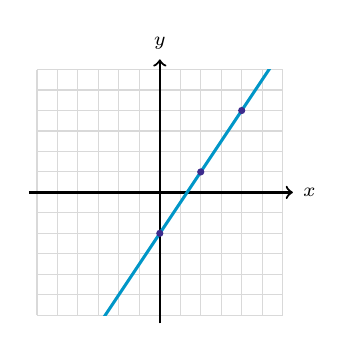
\begin{tikzpicture}[scale=0.26]
\draw[gray!30,thin] (-6,-6) grid (6,6);
\draw[->,thick] (-6.4,0)--(6.5,0) node[right,font=\scriptsize]{$x$};
\draw[->,thick] (0,-6.4)--(0,6.5) node[above,font=\scriptsize]{$y$};
\begin{scope}\clip (-6,-6) rectangle (6,6);
\draw[fmkey,line width=1.1pt] (-7,-12.500)--(7,8.500);
\end{scope}
\fill[fmtitle] (0.0,-2.0) circle (5pt);
\fill[fmtitle] (2.0,1.0) circle (5pt);
\fill[fmtitle] (4.0,4.0) circle (5pt);
\end{tikzpicture}\end{minipage}\end{watchme}
\needspace{6.2cm}\par\vspace{3mm}\noindent \begin{minipage}[t]{0.48\linewidth}\raggedright{\color{fmturn}\bfseries 23.}\ Graph $y = 2x - 3$.\par\vspace{1mm}\centering 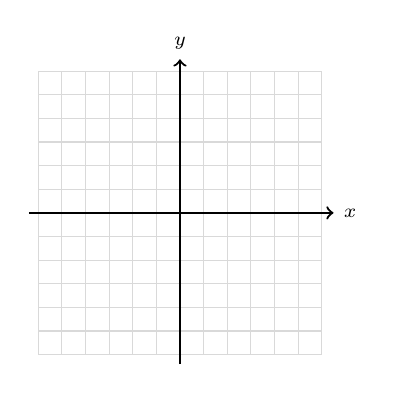
\begin{tikzpicture}[scale=0.3]
\draw[gray!30,thin] (-6,-6) grid (6,6);
\draw[->,thick] (-6.4,0)--(6.5,0) node[right,font=\scriptsize]{$x$};
\draw[->,thick] (0,-6.4)--(0,6.5) node[above,font=\scriptsize]{$y$};
\begin{scope}\clip (-6,-6) rectangle (6,6);
\end{scope}
\end{tikzpicture}\end{minipage}\hfill \begin{minipage}[t]{0.48\linewidth}\raggedright{\color{fmturn}\bfseries 24.}\ Graph $y = -\dfrac{1}{2}x + 4$.\par\vspace{1mm}\centering 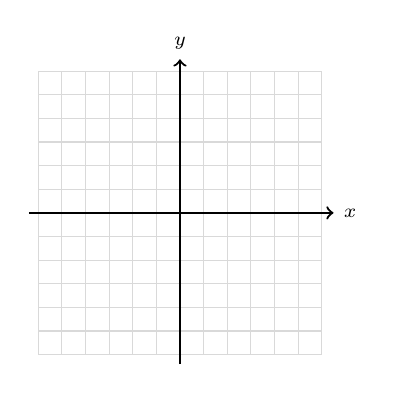
\begin{tikzpicture}[scale=0.3]
\draw[gray!30,thin] (-6,-6) grid (6,6);
\draw[->,thick] (-6.4,0)--(6.5,0) node[right,font=\scriptsize]{$x$};
\draw[->,thick] (0,-6.4)--(0,6.5) node[above,font=\scriptsize]{$y$};
\begin{scope}\clip (-6,-6) rectangle (6,6);
\end{scope}
\end{tikzpicture}\end{minipage}\par
\needspace{6.2cm}\par\vspace{3mm}\noindent \begin{minipage}[t]{0.48\linewidth}\raggedright{\color{fmturn}\bfseries 25.}\ Graph $y = \dfrac{2}{3}x - 1$.\par\vspace{1mm}\centering 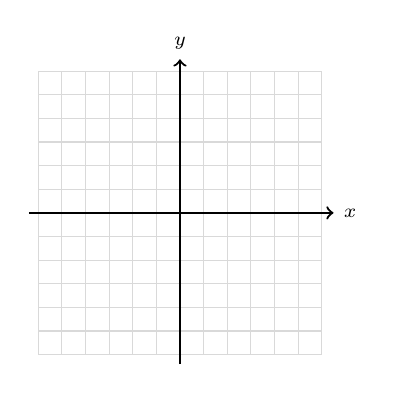
\begin{tikzpicture}[scale=0.3]
\draw[gray!30,thin] (-6,-6) grid (6,6);
\draw[->,thick] (-6.4,0)--(6.5,0) node[right,font=\scriptsize]{$x$};
\draw[->,thick] (0,-6.4)--(0,6.5) node[above,font=\scriptsize]{$y$};
\begin{scope}\clip (-6,-6) rectangle (6,6);
\end{scope}
\end{tikzpicture}\end{minipage}\hfill \begin{minipage}[t]{0.48\linewidth}\raggedright{\color{fmturn}\bfseries 26.}\ Graph $y = -3x + 2$.\par\vspace{1mm}\centering 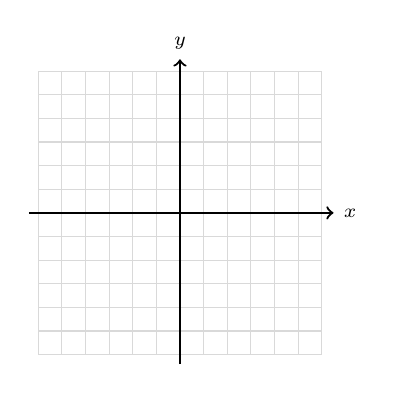
\begin{tikzpicture}[scale=0.3]
\draw[gray!30,thin] (-6,-6) grid (6,6);
\draw[->,thick] (-6.4,0)--(6.5,0) node[right,font=\scriptsize]{$x$};
\draw[->,thick] (0,-6.4)--(0,6.5) node[above,font=\scriptsize]{$y$};
\begin{scope}\clip (-6,-6) rectangle (6,6);
\end{scope}
\end{tikzpicture}\end{minipage}\par
\needspace{9cm}\topicbar{Type 6 \quad Linear Functions in Real Life}
\begin{watchme}\textbf{A gym charges a \$20 sign-up fee plus \$5 per visit. Write a function for the cost $C$ after $x$ visits. What do 8 visits cost?}\par\vspace{1mm}The \textbf{starting amount} is $b$. The amount added \textbf{each time} is the slope $m$.\par\vspace{1mm}
\renewcommand{\arraystretch}{2.0}\begin{tabular}{@{}l l@{}}
\textbf{Step 1 \ Starting amount} & $b = 20$\\
\textbf{Step 2 \ Rate (per visit)} & $m = 5$\\
\textbf{Step 3 \ Write and use it} & $C = 5x + 20$; \ $C = 5 \cdot 8 + 20 = 60$\\
\textbf{Answer} & $\boldsymbol{C = 5x + 20}$; \ 8 visits cost $\boldsymbol{\$60}$
\end{tabular}\end{watchme}
\needspace{3.7cm}\par\vspace{3mm}\noindent \begin{minipage}[t][3.2cm]{0.48\linewidth}\raggedright{\color{fmturn}\bfseries 27.}\ A taxi charges \$3 to start plus \$2 per mile. Write the cost $C$ for $x$ miles. Find the cost of a 12-mile ride.\par\vfill\hfill Answer:\ \rule{3.2cm}{0.4pt}\end{minipage}\hfill \begin{minipage}[t][3.2cm]{0.48\linewidth}\raggedright{\color{fmturn}\bfseries 28.}\ A candle is 30 cm tall and burns 2 cm per hour. Write its height $h$ after $t$ hours. When does it burn out?\par\vfill\hfill Answer:\ \rule{3.2cm}{0.4pt}\end{minipage}\par
\needspace{3.7cm}\par\vspace{3mm}\noindent \begin{minipage}[t][3.2cm]{0.48\linewidth}\raggedright{\color{fmturn}\bfseries 29.}\ A plant is 4 inches tall and grows 1.5 inches per week. Write its height $h$ after $w$ weeks. How tall is it after 6 weeks?\par\vfill\hfill Answer:\ \rule{3.2cm}{0.4pt}\end{minipage}\hfill \begin{minipage}[t][3.2cm]{0.48\linewidth}\raggedright{\color{fmturn}\bfseries 30.}\ Mia has \$200 and spends \$15 each week. Write her money $M$ after $w$ weeks. What do the slope and $y$-intercept mean?\par\vfill\hfill Answer:\ \rule{3.2cm}{0.4pt}\end{minipage}\par
\end{document}
